%% Body-free VLDB/acmart placement check for E3--E5.
%% Uses the paper's acmart + pvldb. No prose, no shared entry-point edits.
\documentclass[sigconf,nonacm,review]{acmart}
\usepackage{pvldb}
\settopmatter{printacmref=false,printfolios=true}
\usepackage{graphicx}
\usepackage{subfigure}
% main.tex uses subfigcapskip=-7pt. That skip covered the panel xlabel on this
% compile, so the preview keeps the caption just under the panel.
\setlength{\subfigcapskip}{1pt}
\setlength{\subfigbottomskip}{0pt}
\setlength{\abovecaptionskip}{0.2cm}
\setlength{\belowcaptionskip}{-0.15cm}
\graphicspath{%
  {../figures/e3/}%
  {../figures/e4a/}%
  {../figures/e4b/}%
  {../figures/e4c/}%
  {../figures/e5/}%
}
\title{E3--E5 figure placement}
\author{Placement}
\renewcommand{\shortauthors}{Placement}
\providecommand{\shorttitle}{E3--E5 figure placement}
\begin{document}
\maketitle
\typeout{COLUMNWIDTH=\the\columnwidth}
\typeout{TEXTWIDTH=\the\textwidth}
\typeout{TEXTHEIGHT=\the\textheight}
% One stored float per column. The as-compiled queue dropped
% TREC-COVID n=100 and E4c, and stacked E4b under E4a until the
% caption crossed the bottom margin. Flush after each float.
\let\VPendfigure\endfigure
\def\endfigure{\VPendfigure\clearpage}
% E3 scale scaffold. Single-column container copied from the original
% fig:exp4-topk (exp.tex, Figure 8): legend above, panels at 0.25\columnwidth.
% SW / LT / Full / LIMIT / predicted / measured are set here, not inside the PDFs.
% Not inserted into the paper. Graphic path: figures/e3/
\begin{figure}[t]
  % Local to this float. The old paper sets \subfigcapskip=-7pt, which
  % pulls n / 10k under the subcaption. Do not inherit that value.
  \setlength{\subfigcapskip}{1pt}
  \centering
  
\includegraphics[width=\columnwidth]{e3-legend.pdf}\par
  \vspace{-0.45em}
  % Two short lines: a single line does not fit in 0.25 column.
  % Fig.~8 uses \hspace{-2.6ex}. At this panel's margins that shift
  % covers the following panel's "10k" (sigconf preview), so the
  % four boxes sit edge to edge instead.
  \newcommand{\eiiicap}[2]{\protect\shortstack{\scriptsize #1\\#2}}%
  \subfigure[\eiiicap{SW, Full}{predicted}]{%
    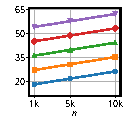
\includegraphics[width=0.25\columnwidth]{e3-sw-full-predicted.pdf}}%
  \subfigure[\eiiicap{SW, LIMIT}{predicted}]{%
    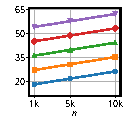
\includegraphics[width=0.25\columnwidth]{e3-sw-limit10-predicted.pdf}}%
  \subfigure[\eiiicap{LT, Full}{predicted}]{%
    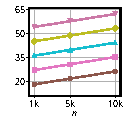
\includegraphics[width=0.25\columnwidth]{e3-lt-full-predicted.pdf}}%
  \subfigure[\eiiicap{LT, LIMIT}{predicted}]{%
    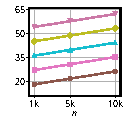
\includegraphics[width=0.25\columnwidth]{e3-lt-limit10-predicted.pdf}}%
  \\[0.15em]
  \subfigure[\eiiicap{SW, Full}{measured}]{%
    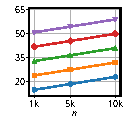
\includegraphics[width=0.25\columnwidth]{e3-sw-full-measured.pdf}}%
  \subfigure[\eiiicap{SW, LIMIT}{measured}]{%
    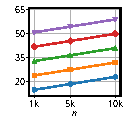
\includegraphics[width=0.25\columnwidth]{e3-sw-limit10-measured.pdf}}%
  \subfigure[\eiiicap{LT, Full}{measured}]{%
    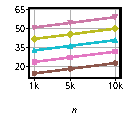
\includegraphics[width=0.25\columnwidth]{e3-lt-full-measured.pdf}}%
  \subfigure[\eiiicap{LT, LIMIT}{measured}]{%
    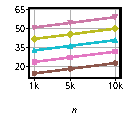
\includegraphics[width=0.25\columnwidth]{e3-lt-limit10-measured.pdf}}%
  \caption{Synthetic scale scaffold, not a measured token cost.
  Top row predicted, bottom row measured.
  Left legend entries are the SW series $(k,h)$; right entries are the LT series.
  The horizontal position is linear in $n\in\{1\mathrm{k},5\mathrm{k},10\mathrm{k}\}$;
  the vertical axis is one shared layout scale.
  Panel box is $0.25$ column.}
  \label{fig:e3-scale}
\end{figure}

% E4a. One single-column figure per dataset and n.
% Not inserted into the paper. Graphic path: figures/e4a/
\newcommand{\eFourAnote}{%
  Synthetic layout sample, not an experimental result.
  A star is the predicted configuration and a diamond the measured minimum, both at that configuration's measured height.
  The minimum is over the displayed categories only, not the legal domain.
  Real display points are still deferred.%
}

\begin{figure}[t]
  \centering
  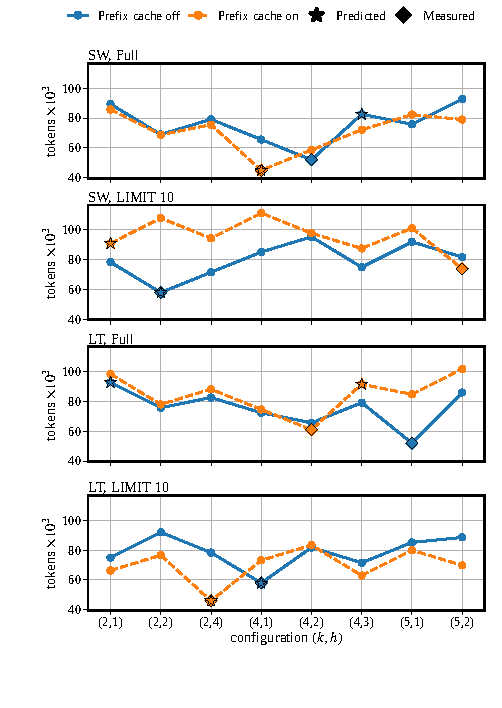
\includegraphics[width=\columnwidth]{e4a-dl20-n100.pdf}
  \caption{DL20, $n{=}100$. \eFourAnote}
  \label{fig:e4a-dl20-n100}
\end{figure}

\begin{figure}[t]
  \centering
  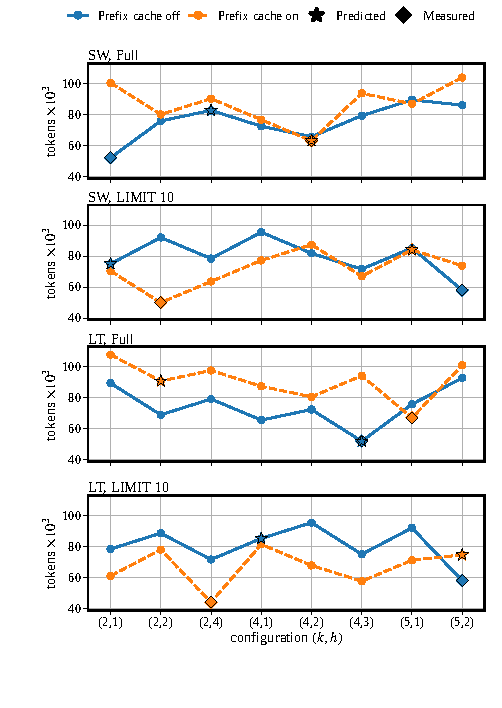
\includegraphics[width=\columnwidth]{e4a-covid-n100.pdf}
  \caption{TREC-COVID, $n{=}100$. \eFourAnote}
  \label{fig:e4a-covid-n100}
\end{figure}

\begin{figure}[t]
  \centering
  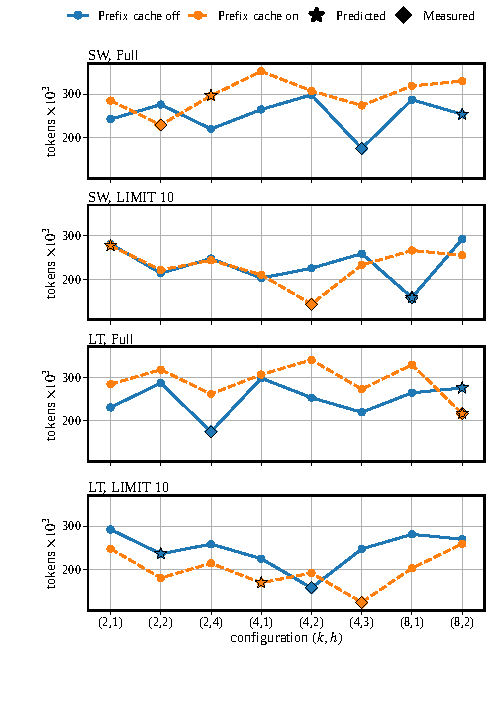
\includegraphics[width=\columnwidth]{e4a-dl20-n500.pdf}
  \caption{DL20, $n{=}500$. \eFourAnote}
  \label{fig:e4a-dl20-n500}
\end{figure}

\begin{figure}[t]
  \centering
  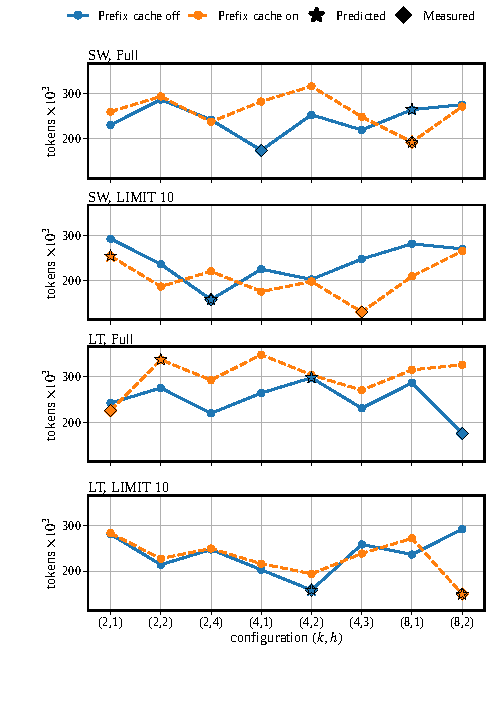
\includegraphics[width=\columnwidth]{e4a-covid-n500.pdf}
  \caption{TREC-COVID, $n{=}500$. \eFourAnote}
  \label{fig:e4a-covid-n500}
\end{figure}

% E4b. Single column, no background bands, no inset.
% Not inserted into the paper. Graphic path: figures/e4b/
\begin{figure}[t]
  \centering
  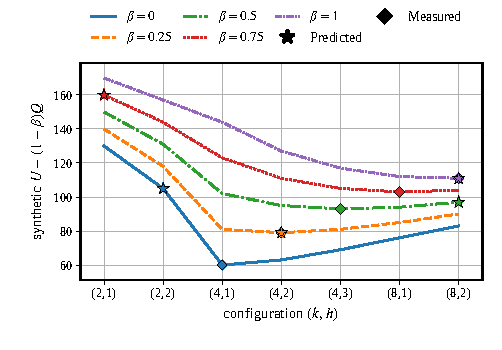
\includegraphics[width=\columnwidth]{e4b-beta.pdf}
  \caption{Synthetic On-cold slice, not a measured cost.
  Each curve is $U-(1-\beta)Q$ at the drawn $\beta$ values.
  A star is the placeholder predicted configuration and a diamond is the measured minimum of that curve; both sit on the curve.}
  \label{fig:e4b-beta}
\end{figure}

\let\endfigure\VPendfigure
% E4c. Single-column 2 by 2. Not inserted into the paper.
% Graphic path: figures/e4c/
\begin{figure}[t]
  \centering
  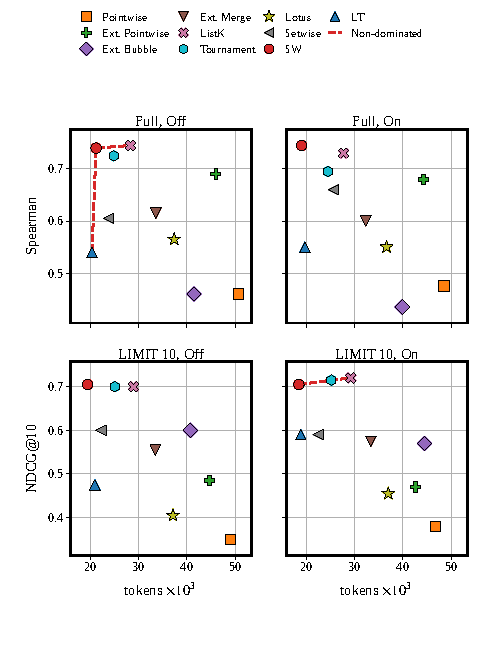
\includegraphics[width=\columnwidth]{e4c-quality-cost.pdf}
  \caption{Synthetic layout sample, not an experimental result.
  Each point is one method.
  The DL20 and COVID dataset-level placeholders are averaged with equal weight $1/2$; cost and quality are averaged separately.
  Query rows were not stored, so this is not a six-query mean and no per-query cloud is drawn.
  The two Full panels share Spearman limits, the two LIMIT~10 panels share NDCG@10 limits, and all four share the token axis.
  ListK Fig.~4 calls its red dotted curve a Pareto frontier and also runs that curve off the plotted points.
  The red dashed segments here join only non-dominated means, lower equivalent tokens and higher quality, and they stop at those means.
  They are a descriptive set, not a fit and not a significance claim.
  Full, Off joins LT, SW, and ListK.
  LIMIT~10, On joins SW, Tournament, and ListK.
  Full, On and LIMIT~10, Off each have one non-dominated mean (SW), so no segment is drawn.}
  \label{fig:e4c-quality-cost}
\end{figure}

% E5. Full-width 4 by 2. The panel interior is the previously accepted
% composition: equal LIMIT slots, Full on a broken-off axis, not joined.
% Not inserted into the paper. Graphic path: figures/e5/
\begin{figure*}[t]
  \centering
  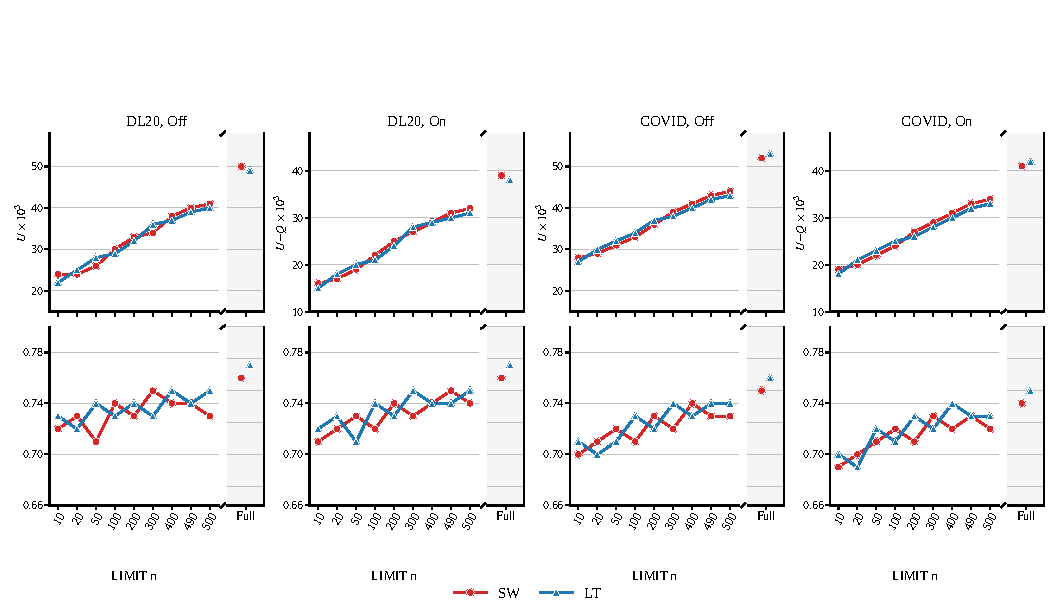
\includegraphics[width=\textwidth]{e5-limit-sweep.pdf}
  \caption{Synthetic placeholder, not a measured advantage.
  Full is a separate mode and is not joined to LIMIT~500, and it is not $K{=}510$.
  Off is equivalent input $U$; On-cold is $U{-}Q$ at $\beta{=}0$.
  The two cache states do not share a cost scale.
  Slots are equally spaced contract positions, not linear in $n$.}
  \label{fig:e5-limit-sweep}
\end{figure*}

\clearpage
\end{document}
